
\documentclass[12pt, a4paper]{article}


%%%% Encodings

\usepackage[utf8]{inputenc} % encoding
\usepackage[english]{babel} % use special characters and also translates some elements within the document.

%%%% Misc

\usepackage{hyperref}       % Hyperlinks \url{url} or \href{url}{name}
\usepackage{parskip}        % \par starts on left (not idented)
\usepackage{tocbibind}      % Adds the bibliography to the table of contents (automatically)

% \usepackage[document]{ragged2e}  % Left-aligned (whole document)
% \begin{...} ... \end{...}   flushleft, flushright, center

%%%% Abstract

\usepackage{abstract}       % Abstract

% http://www.ctex.org/documents/packages/special/abstract.pdf
\renewcommand{\absnamepos}{flushleft} % \begin{abstract} \noindent ... \end{abstract}
\setlength{\absleftindent}{0pt}
\setlength{\absrightindent}{0pt}

%%%% Graphics

\usepackage{graphicx}
\graphicspath{ {./images/} } % directory to look up for graphics

% \begin{figure}[h]
%   \centering
%   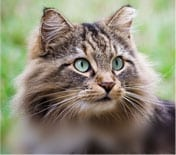
\includegraphics[scale=0.5]{cat}  % [width=\textwidth, height=4cm],
%   \caption{Example of a cat}
%   \label{fig:cat}
% \end{figure}

%%%% Math

\usepackage{amsmath}        % Math
\usepackage{amssymb}        % New symbols http://milde.users.sourceforge.net/LUCR/Math/mathpackages/amssymb-symbols.pdf
\usepackage{bm}             % $\bm{D + C}$

\usepackage{amsthm} % Math, \newtheorem, \proof, etc
% \begin{theorem}\label{t:label}  ...  \end{theorem}
% \begin{proof} ... \end{proof}
\theoremstyle{plain} % default
\newtheorem{theorem}{Theorem}[section]
\newtheorem{corollary}{Corollary}[theorem]  % Numering depends on the current section (instead of global)
\newtheorem{lemma}[theorem]{Lemma} % Shares numeration with theorem.
\theoremstyle{definition}
\newtheorem{definition}{Definition}[section]
\theoremstyle{remark}
\newtheorem*{remark}{Remark}

% Defines a new environment to write your or claim - proof
\newenvironment{claim}[1]{\par\noindent\underline{Claim:}\space#1}{}
\newenvironment{claimproof}[1]{\par\noindent\underline{Proof:}\space#1}{\hfill $\blacksquare$}

%%%% Code/Pseudo-code

\usepackage{minted} % Code listing
% \mint{html}|<h2>Something <b>here</b></h2>|
% \inputminted{octave}{BitXorMatrix.m}

%\begin{listing}[H]
  %\begin{minted}[xleftmargin=20pt,linenos,bgcolor=codegray]{haskell}
  %\end{minted}
  %\caption{Example of a listing.}
  %\label{lst:example} % You can reference it by \ref{lst:example}
%\end{listing}

\newcommand{\code}[1]{\texttt{#1}} % Define \code{foo.hs} environment

\usepackage[vlined,ruled]{algorithm2e} % pseudo-code http://tug.ctan.org/macros/latex/contrib/algorithm2e/doc/algorithm2e.pdf

%%%% Colors

\usepackage{xcolor}         % Colours \definecolor, \color{codegray}
\definecolor{codegray}{rgb}{0.9, 0.9, 0.9}
% \color{codegray} ... ...
% \textcolor{red}{easily}

%%%% Math

%\makeglossaries % before entries

%\newglossaryentry{latex}{
    %name=latex,
    %description={Is a mark up language specially suited
    %for scientific documents}
%}

% Referene to a glossary \gls{latex}
% Print glossaries \printglossaries

\usepackage[acronym]{glossaries} %

% \acrshort{name}
% \acrfull{name}
% \newacronym{foo}{arcshort}{acrfull}

\usepackage{enumitem}


\usepackage{fancyhdr}
\pagestyle{fancy}
\fancyhf{}
\rhead{TODO}
\lhead{TODO}
\rfoot{Page \thepage}

\title{%
  \vspace{-10ex}
  \Large{Algorithmic Methods for Mathematical Models (AMMM)} \\
  \large{Lab Session 3 - More on Mixed Integer Linear Programs}
}
\author{%
  Arnau Abella \\
  \large{Universitat Polit\`ecnica de Catalunya}
}
\date{\today}

\begin{document}
\maketitle

\vspace{10ex}
\begin{enumerate}[label=(\alph*)]
    \item Implement the P3 model in OPL and solve it using CPLEX with the following data file.

    The OPL model can be found at \code{computer.mod} file.

    The results of the execution are the following

    % \inputminted{modula2}{computer.mod}
    \begin{minted}{text}
Problem: test.dat
262414.256133333

Task - Computer
[1,0,0,]
[0,0,1,]
[0,1,0,]
[1,0,0,]

Thread - Core
[0,1,0,0,0,0,0,0,0,]
[1,0,0,0,0,0,0,0,0,]
[0,0,0,0,0,0,1,0,0,]
[0,0,0,0,0,0,0,1,0,]
[0,0,0,1,0,0,0,0,0,]
[0,0,0,0,0,1,0,0,0,]
[1,0,0,0,0,0,0,0,0,]
[1,0,0,0,0,0,0,0,0,]
CPU 1 loaded at 0.483938801
CPU 2 loaded at 0.410988458
CPU 3 loaded at 0.532826052
    \end{minted}

    \newpage

    \item Generate instances of increasing size with the instance generator script and use the \textit{P3} model to solve them.

    The OPL script can be found at \code{script.mod} file.

    I will only attach the results of the small data (\code{small.dat}) but the script is prepared to also run the medium data (\code{mid.dat}) and big data (\code{big.dat}).

    \begin{minted}{text}
Problem: small_0.dat
21134171.221917309

Task - Computer
[0,1,0,0,0,]
[1,0,0,0,0,]
[0,0,0,0,1,]
[0,0,1,0,0,]
[...]

Thread - Core
[0,0,0,1,0,0,0,0,0,0,]
[0,0,1,0,0,0,0,0,0,0,]
[0,0,0,1,0,0,0,0,0,0,]
[0,0,0,0,1,0,0,0,0,0,]
[0,0,1,0,0,0,0,0,0,0,]
[...]

CPU 1 loaded at 0.455212688
CPU 2 loaded at 0.320378826
CPU 3 loaded at 0.270715188
CPU 4 loaded at 0.684153368
CPU 5 loaded at 0.670319832
    \end{minted}

    \item Modify the \textit{P3} model to maximize the number of computers with all their cores empty (\textit{P3a}).

    The OPL model can be found at \code{computer2.mod} file.

    \newpage

    \item Compare both models \textit{(P3 and P3a)} in terms of number of variables, constraints and execution time for the generated instances.

    \begin{table}[H]
      \begin{center}
        \begin{tabular}{l | c r}
          & P3 & P3a \\
          \hline
          Constraint & 32 & 38 \\
          Variables & 85 & 88 \\
          CPU Time & 0.185 & 0.16 \\
        \end{tabular}
      \end{center}
      \caption{Comparison on \code{test.dat}}
    \end{table}

    \begin{table}[H]
      \begin{center}
        \begin{tabular}{l | c r}
          & P3 & P3a \\
          \hline
          Constraint &  215 & 225 \\
          Variables & 1101 & 1106 \\
          CPU Time & 5.27 & 3.90 \\
        \end{tabular}
      \end{center}
      \caption{Comparison on \code{small.dat}}
    \end{table}

\end{enumerate}


\end{document}
